\documentclass[11pt,a4paper]{article}
\usepackage[utf8]{inputenc}
\usepackage[T1]{fontenc}
\usepackage{tgpagella}
\usepackage[spanish]{babel}
\usepackage{geometry}
\usepackage{booktabs}
\usepackage{xcolor}
\usepackage{titlesec}
\usepackage{fancyhdr}
\usepackage[parfill]{parskip}
\usepackage[expansion=false]{microtype}
\usepackage{hyperref}
\usepackage{setspace}
\usepackage{needspace}
\usepackage{graphicx}
\usepackage[table]{xcolor}
\usepackage{booktabs}
\usepackage{array}
\widowpenalty=10000
\clubpenalty=10000
\displaywidowpenalty=10000

\geometry{top=3.0cm,bottom=3.0cm,left=3.5cm,right=3.5cm}
\setlength{\parskip}{0.65em}
\setlength{\parindent}{0em}

\definecolor{azulai}{RGB}{30,80,140}
\definecolor{doradoai}{RGB}{140,90,0}
\definecolor{grisai}{RGB}{70,70,70}

\titleformat{\section}{\Large\bfseries\color{azulai}}{}{0em}{}[{\color{azulai}\titlerule[0.5pt]\nopagebreak[4]}]
\titlespacing*{\section}{0pt}{1.8em}{0.8em}
\titleformat{\subsection}{\large\bfseries\color{doradoai}}{}{0em}{}[{\nopagebreak[4]}]
\titlespacing*{\subsection}{0pt}{1.4em}{0.5em}
\titleformat{\subsubsection}{\normalsize\bfseries\color{grisai}}{}{0em}{}[{\nopagebreak[4]}]
\titlespacing*{\subsubsection}{0pt}{1.0em}{0.3em}

\pagestyle{fancy}\fancyhf{}
\rhead{\textcolor{grisai}{\small Maite Barragan — Arquitectura Interna}}
\lhead{\textcolor{grisai}{\small Casas por signo}}
\cfoot{\textcolor{grisai}{\small\thepage}}
\renewcommand{\headrulewidth}{0.3pt}

\hypersetup{colorlinks=true,linkcolor=azulai,urlcolor=azulai}
\setstretch{1.45}
\tolerance=1500
\emergencystretch=4em

\begin{document}

% ── Portada ──────────────────────────────────────────────────────────────────
\begin{titlepage}
  \centering
  \vspace*{1.5cm}
  {\Huge\bfseries\color{azulai} Casas por signo}\\[0.5cm]
  {\large\color{grisai} Arquitectura Interna}\\[0.3cm]
  {\small\itshape\color{grisai} Organización de la vida: ejes, distribución e interceptaciones}\\[2cm]
  {\huge\color{doradoai} Maite Barragan}\\[1.5cm]
  {\Large 07/01/1971 \quad 12:15}\\[0.3cm]
  {\Large Pamplona, España}\\[0.3cm]
  {\normalsize Lat: 42.8157° \quad Lon: -1.6522° \quad UTC+01:00}\\[0.3cm]
  {\normalsize Ascendente: Aries 6°18' \quad
    MC: Capricornio 3°11'}\\[2cm]
  \begin{tabular}{ll}
    \textbf{ASC (Casa 1):}  & Aries 6°18' \\
    \textbf{DSC (Casa 7):}  & Libra 6°18' \\
    \textbf{MC (Casa 10):}  & Capricornio 3°11' \\
    \textbf{IC (Casa 4):}   & Cáncer 3°11' \\
  \end{tabular}\\[2cm]
  \vfill
  {\small Generado el 20/05/2026}
\end{titlepage}

\tableofcontents
\newpage

\begin{center}
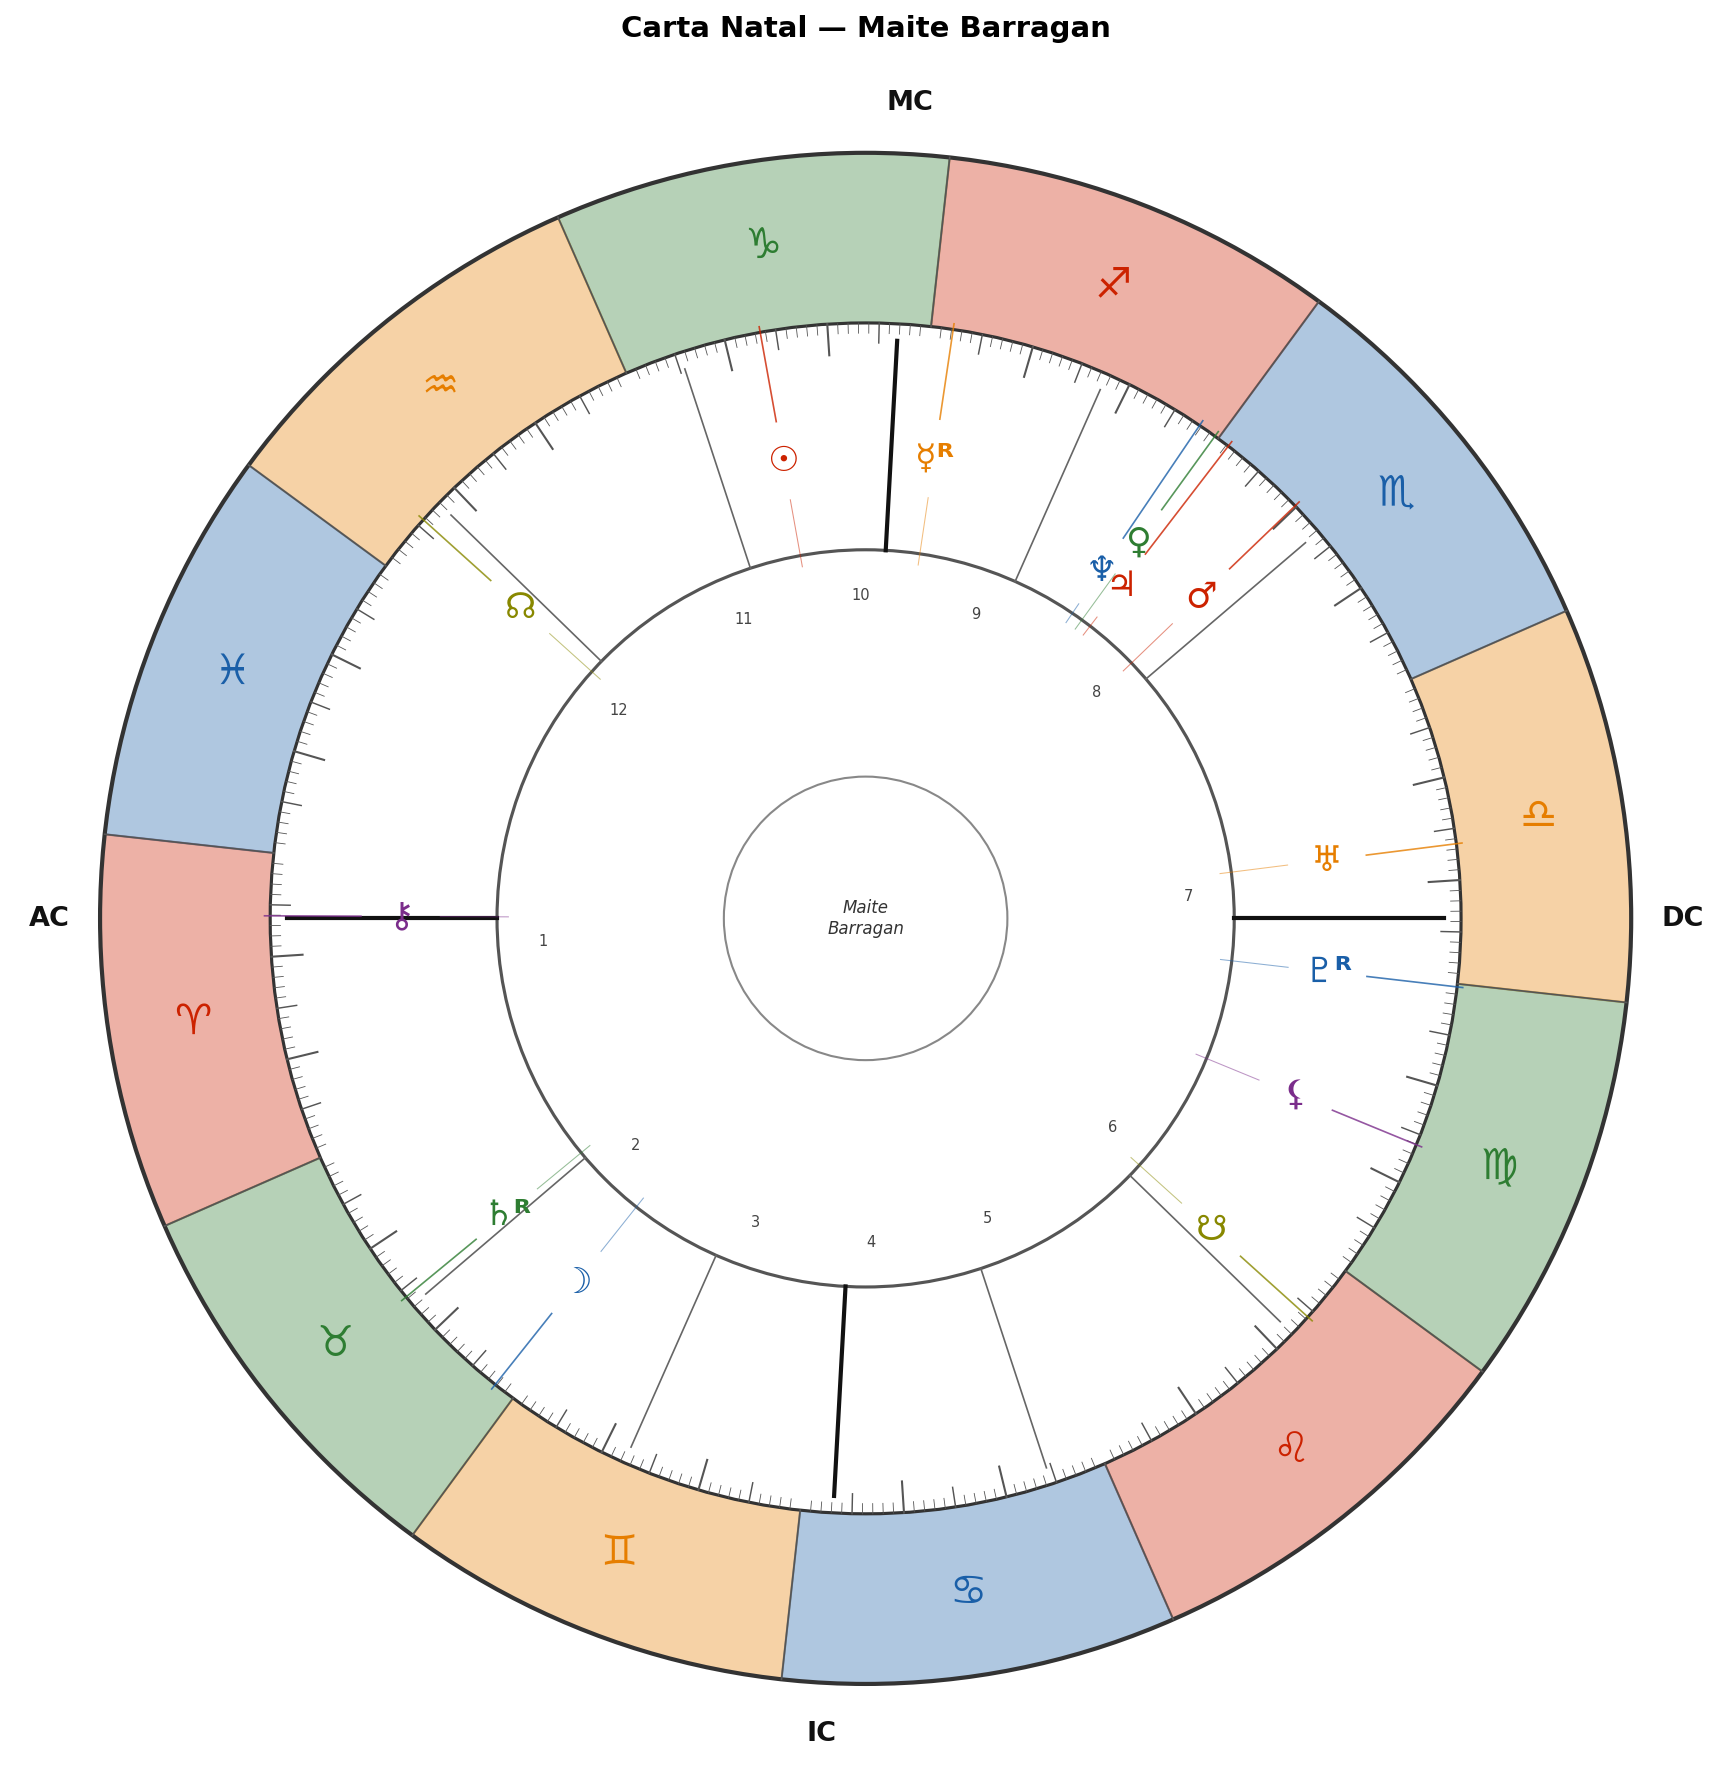
\includegraphics[width=0.88\textwidth]{rueda_casas.png}
\end{center}

\newpage

% ── Datos de referencia ───────────────────────────────────────────────────────
\section{Datos de referencia}

\begin{center}
\begin{tabular}{rllll}
  \toprule
  \textbf{Casa} & \textbf{Área} & \textbf{Signo} & \textbf{Cúspide} & \textbf{Planetas} \\
  \midrule
  1 & Identidad y presencia & Aries & 6°18' & Saturno \\
  2 & Recursos y seguridad & Tauro & 16°48' & Luna \\
  3 & Comunicación y entorno cercano & Géminis & 12°23' & — \\
  4 & Base y hogar & Cáncer & 3°11' & — \\
  5 & Expresión y creatividad & Cáncer & 24°31' & — \\
  6 & Vida cotidiana y salud & Leo & 22°06' & Plutón \\
  7 & Vínculos y relaciones & Libra & 6°18' & Urano \\
  8 & Transformación y profundidad & Escorpio & 16°48' & Venus, Marte, Júpiter, Neptuno \\
  9 & Horizonte y expansión & Sagitario & 12°23' & Mercurio \\
  10 & Dirección y proyección & Capricornio & 3°11' & Sol \\
  11 & Redes y colectivo & Capricornio & 24°31' & — \\
  12 & Mundo interior & Acuario & 22°06' & — \\
  \bottomrule
\end{tabular}
\end{center}

\vspace{0.3cm}\textbf{Signos interceptados:} Virgo (Casa 6); Piscis (Casa 12)

\newpage

% ── Interpretación ────────────────────────────────────────────────────────────
\section{Interpretación — Arquitectura Interna}

\begin{center}
{\small\itshape
No se trata de describir la personalidad.\\ Se trata de mostrar cómo está organizada la vida y qué implica esa organización.
}
\end{center}

\vspace{0.5cm}
\Needspace{5\baselineskip}

% ── 1. Estructura general ──────────────────────────────────────────────────────
\needspace{3\baselineskip}
\subsection{1. Estructura general de casas}

La mayor parte de los planetas principales (7 de 10) están en las casas 7–12. Esto suele indicar que buena parte de tu energía se despliega a través del contacto con otras personas, los vínculos, el mundo exterior y la dimensión social o colectiva.

La mayor parte de los planetas están en el sector occidental de la carta (casas 6–11: 8). Esto suele mostrar una vida donde los vínculos, las respuestas del entorno y lo que ocurre con otras personas tienen mucho peso.

Casas con mayor concentración de planetas:
Casa 8 (Transformación y profundidad): Venus, Marte, Júpiter, Neptuno — área especialmente importante

Las casas con más planetas señalan áreas de vida donde se concentra mucha atención, movimiento interno y aprendizaje. No significa que sean las únicas importantes, pero sí que suelen tener más peso en tu manera de vivir, decidir y organizarte.

\vspace{0.5cm}
\Needspace{5\baselineskip}

% ── 2. Ejes principales ───────────────────────────────────────────────────────
\needspace{3\baselineskip}
\subsection{2. Ejes principales}

\subsubsection*{Ascendente — Aries (6°18')}
Con Ascendente en Aries, sueles entrar en la vida de forma directa y rápida. Tiendes a actuar antes de tener todas las respuestas, y muchas veces descubres el camino mientras ya estás avanzando.

Las demás personas suelen percibirte como una persona con iniciativa, energía o capacidad para moverse hacia adelante. A veces, sin embargo, la velocidad puede hacer que te cueste parar y registrar realmente lo que estás sintiendo o viviendo.

\subsubsection*{Descendente — Libra}
Con Descendente en Libra, tiendes a buscar relaciones equilibradas y recíprocas. Necesitas sentir que hay diálogo, escucha y cierta armonía en el vínculo.

Suele haber mucha importancia en la capacidad de llegar a acuerdos y construir desde el respeto mutuo, aunque a veces puedes evitar el conflicto incluso cuando sería necesario atravesarlo.

\subsubsection*{Medio Cielo — Capricornio (3°11')}
Con Medio Cielo en Capricornio, sueles orientarte profesionalmente de forma seria, constante y construida a largo plazo. Muchas veces existe necesidad de consolidar algo sólido con el tiempo.

Aquí suele haber disciplina, responsabilidad y capacidad de esfuerzo sostenido. El reconocimiento suele llegar lentamente, pero con más estabilidad y profundidad.

\subsubsection*{Fondo del Cielo — Cáncer}
Con Fondo del Cielo en Cáncer, tu base interior suele estar muy ligada a la necesidad de refugio emocional, protección y pertenencia. Muchas veces necesitas sentirte en casa emocionalmente para poder relajarte de verdad.

Aquí suele haber mucha sensibilidad en lo íntimo y en los vínculos cercanos. Muchas veces recuperas energía cuando sientes cuidado, confianza y seguridad emocional.

\subsubsection*{La relación entre los ejes}
Ascendente (Aries, Fuego) y Medio Cielo (Capricornio, Tierra) están en elementos que pueden crear tensión. Puede haber diferencia entre cómo entras en las situaciones y lo que necesitas construir o mostrar hacia fuera. A veces esto hace que las demás personas perciban una parte de ti mientras tu dirección profunda va por otro lugar.

\vspace{0.5cm}
\Needspace{5\baselineskip}

% ── 3. Signos por casas ───────────────────────────────────────────────────────
\needspace{3\baselineskip}
\subsection{3. Distribución de signos por casas}

\subsubsection*{Casa 1 — Identidad y presencia · Aries}
La Casa 1 habla de cómo entras en la vida y de la impresión que sueles generar de forma espontánea. Tiene relación con la presencia, el cuerpo y la manera en que tiendes a posicionarte cuando algo comienza.

Con Aries en la cúspide, esta área de la vida suele moverse rápido. Tiendes a entrar antes de tenerlo todo claro y muchas veces necesitas descubrir sobre la marcha qué hacer con lo que aparece.

Aquí suele haber iniciativa, impulso y necesidad de avanzar, aunque a veces puede costar sostener lo empezado cuando desaparece la motivación inicial.

Planetas en esta casa: Saturno. Este planeta añade una capa importante a la manera en que vives esta área.

\subsubsection*{Casa 2 — Recursos y seguridad · Tauro}
La Casa 2 muestra tu relación con la seguridad, los recursos y aquello que necesitas para sentir estabilidad. Aquí aparecen tanto lo material como la sensación interna de sostén.

Con Tauro en la cúspide, esta parte de la vida necesita tiempo para asentarse. No sueles moverte deprisa aquí, pero cuando algo echa raíces puede mantenerse durante mucho tiempo.

La estabilidad tiene mucha importancia en este ámbito, aunque a veces puede costar hacer cambios incluso cuando ya serían necesarios.

Planetas en esta casa: Luna. Este planeta añade una capa importante a la manera en que vives esta área.

\subsubsection*{Casa 3 — Comunicación y entorno cercano · Géminis}
La Casa 3 se relaciona con la comunicación cotidiana, el pensamiento habitual y el entorno cercano. Habla de cómo procesas lo inmediato y de la manera en que intercambias información con lo que te rodea.

Con Géminis en la cúspide, esta área suele vivirse desde la curiosidad, el movimiento y la necesidad de variedad. Tiendes a aprender rápido y a conectar fácilmente con distintas ideas o personas.

Aquí suele haber agilidad mental y facilidad para adaptarte, aunque mantener una única dirección durante mucho tiempo puede hacerse más difícil.

\subsubsection*{Casa 4 — Base y hogar · Cáncer}
La Casa 4 habla de la base emocional y del lugar interno desde el que necesitas sostenerte. Tiene relación con el hogar, las raíces, la intimidad y aquello que te ayuda a sentir refugio.

Con Cáncer en la cúspide, esta parte de la vida suele vivirse de forma muy sensible y personal. Necesitas sentir seguridad emocional antes de abrirte o avanzar realmente en este ámbito.

Aquí tiene mucha importancia la protección, el cuidado y la sensación de pertenencia, aunque a veces puedes cerrarte si no sientes suficiente confianza.

\subsubsection*{Casa 5 — Expresión y creatividad · Cáncer}
La Casa 5 muestra cómo tiendes a expresarte cuando hay espacio para hacerlo libremente. Aquí aparece la creatividad, el disfrute, el impulso de crear y aquello que nace desde ti sin obligación.

Con Cáncer en la cúspide, esta parte de la vida suele vivirse de forma muy sensible y personal. Necesitas sentir seguridad emocional antes de abrirte o avanzar realmente en este ámbito.

Aquí tiene mucha importancia la protección, el cuidado y la sensación de pertenencia, aunque a veces puedes cerrarte si no sientes suficiente confianza.

\subsubsection*{Casa 6 — Vida cotidiana y salud · Leo}
La Casa 6 se relaciona con la vida cotidiana, los hábitos y la manera en que cuidas tu energía en el día a día. También habla de la relación con el trabajo cotidiano y con aquello que ayuda a sostener equilibrio y continuidad.

Con Leo en la cúspide, esta área suele cobrar fuerza cuando puedes expresarte con creatividad y sentir que lo que haces tiene valor o impacto. Suele haber bastante energía en este ámbito cuando puedes mostrarte con autenticidad.

Aquí puede aparecer necesidad de reconocimiento o de sentirte visto, aunque a veces el miedo a no recibir respuesta puede hacer que te retraigas más de lo que parece.

Planetas en esta casa: Plutón. Este planeta añade una capa importante a la manera en que vives esta área.

\subsubsection*{Casa 7 — Vínculos y relaciones · Libra}
La Casa 7 habla de los vínculos cercanos y de lo que aparece cuando entras en relación directa con otras personas. Aquí se desarrollan los acuerdos, las asociaciones y las dinámicas de espejo.

Con Libra en la cúspide, esta área suele tomar forma a través de los vínculos y de la relación con otras personas. Necesitas cierto equilibrio o sensación de reciprocidad para sentirte bien aquí.

Aquí suele haber capacidad para dialogar, mediar o buscar armonía, aunque a veces puede costar tomar decisiones sin tener en cuenta constantemente a la otra persona.

Planetas en esta casa: Urano. Este planeta añade una capa importante a la manera en que vives esta área.

\subsubsection*{Casa 8 — Transformación y profundidad · Escorpio}
La Casa 8 se relaciona con los procesos profundos de cambio y transformación. Habla de lo compartido, de lo intenso y de aquello que suele remover capas internas importantes.

Con Escorpio en la cúspide, esta área suele vivirse con intensidad y profundidad. Suele haber dificultad para vivir superficialmente lo que ocurre aquí: cuando algo importa, suele implicar una implicación real.

Aquí suelen aparecer procesos de transformación importantes, aunque a veces también puede haber necesidad de control o dificultad para soltar.

Planetas en esta casa: Venus, Marte, Júpiter, Neptuno. La presencia de varios planetas hace que esta área tenga mucho peso en tu carta. Suele ser un lugar donde se concentran aprendizajes, decisiones y movimiento interno.

\subsubsection*{Casa 9 — Horizonte y expansión · Sagitario}
La Casa 9 muestra la necesidad de ampliar mirada y abrir horizonte. Tiene relación con el aprendizaje profundo, la búsqueda de sentido, los viajes y aquello que expande tu manera de comprender la vida.

Con Sagitario en la cúspide, esta área necesita amplitud, sentido y sensación de crecimiento. Tiendes a moverte mejor cuando sientes que algo te abre horizonte o te permite avanzar más allá de lo conocido.

Aquí suele haber entusiasmo y necesidad de expansión, aunque a veces puede costar concretar o sostener todo lo que se inicia.

Planetas en esta casa: Mercurio. Este planeta añade una capa importante a la manera en que vives esta área.

\subsubsection*{Casa 10 — Dirección y proyección · Capricornio}
La Casa 10 habla de dirección, proyección y construcción visible. Aquí aparece la manera en que buscas desarrollar tu camino y el lugar que deseas ocupar hacia afuera.

Con Capricornio en la cúspide, esta área suele vivirse con responsabilidad y visión a largo plazo. Tiendes a construir despacio, paso a paso, buscando resultados sólidos y duraderos.

Aquí suele haber constancia y capacidad de esfuerzo, aunque a veces puedes cargar con demasiado peso o sentir que nunca es suficiente.

Planetas en esta casa: Sol. Este planeta añade una capa importante a la manera en que vives esta área.

\subsubsection*{Casa 11 — Redes y colectivo · Capricornio}
La Casa 11 se relaciona con los grupos, las redes y los proyectos compartidos. Habla de cómo te vinculas con lo colectivo y de aquello que deseas construir junto a otras personas.

Con Capricornio en la cúspide, esta área suele vivirse con responsabilidad y visión a largo plazo. Tiendes a construir despacio, paso a paso, buscando resultados sólidos y duraderos.

Aquí suele haber constancia y capacidad de esfuerzo, aunque a veces puedes cargar con demasiado peso o sentir que nunca es suficiente.

\subsubsection*{Casa 12 — Mundo interior · Acuario}
La Casa 12 habla del mundo interior y de los procesos que necesitan silencio, retiro o más tiempo para poder comprenderse. Aquí aparecen muchas veces lo inconsciente, el descanso y las partes más difíciles de ver con claridad inmediata.

Con Acuario en la cúspide, esta área suele vivirse de una manera distinta a la habitual. Necesitas libertad, espacio propio o una forma personal de hacer las cosas.

Aquí suele haber necesidad de independencia y mirada amplia, aunque a veces puede costar conectar con lo emocional o con lo más inmediato de este ámbito.



\vspace{0.5cm}
\Needspace{5\baselineskip}

% ── 4. Signos interceptados ───────────────────────────────────────────────────
\needspace{3\baselineskip}
\subsection{4. Signos interceptados}

\subsubsection*{Virgo interceptado — Casa 6}
Virgo está interceptado: la claridad práctica, el orden y la capacidad de ajustar los detalles pueden no estar disponibles desde el principio en ti. Es posible que te cueste ver qué necesita mejora o cómo ordenar lo que está disperso.

En el área donde se encuentra Virgo, puede costarte crear hábitos, establecer método o sostener una atención práctica sin caer en exigencia excesiva. Cuando esta energía se integra, suele aparecer más discernimiento, más precisión y más capacidad para cuidar lo cotidiano.

\subsubsection*{Piscis interceptado — Casa 12}
Piscis está interceptado: la sensibilidad, la apertura y la conexión con lo sutil pueden no expresarse de forma espontánea en ti. Es posible que exista mucha percepción emocional o intuición, pero que cueste confiar en ella.

En el área donde se encuentra Piscis, puede costarte relajarte, soltar el control o permitirte sentir sin intentar entenderlo todo de inmediato. Cuando esta energía se integra, suele aparecer más compasión, más intuición y más capacidad para conectar con lo que no puede explicarse solo desde la lógica.

\subsubsection*{Signos duplicados}
Como consecuencia de las interceptaciones, los signos Capricornio y Cáncer aparecen en dos cúspides consecutivas. Esto puede hacer que dos áreas de tu vida se expresen desde una energía parecida, como si compartieran una misma manera de empezar, reaccionar o tomar forma.



\vspace{0.5cm}
\Needspace{5\baselineskip}

% ── 5. Integración ────────────────────────────────────────────────────────────
\needspace{3\baselineskip}
\subsection{5. Integración}

Ascendente (Aries, Fuego) y Medio Cielo (Capricornio, Tierra) están en elementos que pueden crear tensión. Puede haber diferencia entre cómo entras en las situaciones y lo que necesitas construir o mostrar hacia fuera. A veces esto hace que las demás personas perciban una parte de ti mientras tu dirección profunda va por otro lugar.

La base interna (Cáncer, IC) y la forma en que entras en la vida (Aries, ASC) están en elementos que pueden crear tensión. Puede que lo que te sostiene por dentro no coincida del todo con la manera en que te muestras. Por eso puede ser importante darte tiempo para traducir lo interno hacia fuera sin forzarte a parecer de una forma que no respeta tu raíz.

La Casa 8 (Transformación y profundidad, Escorpio) concentra 4 planetas (Venus, Marte, Júpiter, Neptuno). Esta área tiene mucho peso en tu carta y suele pedir atención especial. Cuando esta parte de la vida está cuidada, puede darte mucha fuerza. Cuando se carga demasiado, también puede absorber más energía de la que parece.

Los signos interceptados (Virgo, Piscis) señalan cualidades que están en ti, pero que quizá no salen de forma inmediata. No están ausentes: necesitan más consciencia, tiempo y práctica para poder expresarse con naturalidad en las áreas donde aparecen.

\vspace{0.5cm}
\Needspace{5\baselineskip}

% ── 6. Orientación práctica ───────────────────────────────────────────────────
\needspace{3\baselineskip}
\subsection{6. Orientación práctica}

\subsubsection*{Desde dónde empezar}
El área con mayor concentración es la Casa 8 (Transformación y profundidad, Escorpio). Puede ayudarte empezar por escuchar lo que sientes antes de exigirte una respuesta externa inmediata.

\subsubsection*{Qué estructurar primero}
La Casa 10 (Dirección y proyección, Capricornio) muestra una parte importante de tu orientación hacia fuera. Lo primero que puede necesitar estructura aquí es crear una base concreta y sostenible antes de intentar crecer demasiado rápido. Sin esa claridad, puede haber mucha energía disponible pero poca dirección de salida.

\subsubsection*{Qué evitar}
Conviene evitar exigirte que tu forma de presentarte (Aries) y tu manera de construir dirección (Capricornio) sean iguales. Son energías diferentes y pueden necesitar ritmos, decisiones y cuidados distintos. Los signos interceptados (Virgo, Piscis) no conviene ignorarlos. Son cualidades disponibles en ti, pero pueden necesitar práctica consciente para no quedar ocultas o poco utilizadas.

\vspace{0.6cm}
Si no atiendes la distribución de las casas, las áreas más cargadas pueden absorber demasiada energía, mientras otras partes de la vida quedan poco cuidadas. La clave no es hacerlo todo con la misma intensidad, sino reconocer dónde hay más peso y qué zonas necesitan una atención más sencilla, clara y constante.

\vspace{0.5cm}
\Needspace{5\baselineskip}
\begin{center}
{\small\itshape\color{grisai}
La astrología se usa aquí como lenguaje simbólico de observación, no como definición de la persona.\\
El sistema es una aproximación funcional, no un diagnóstico.
}
\end{center}

\end{document}
